\documentclass[17pt, a4paper]{extarticle}
\usepackage[unicode]{hyperref}
\usepackage{cmap}
\usepackage{bookmark}
\usepackage{amssymb}
\usepackage{amsmath}
\usepackage{hyperref}
\usepackage{tikz}
\usepackage{pgfplots}
\usepackage{enumitem}
\usepackage{../textbook}

\pgfplotsset{compat=1.17}

\begin{document}

	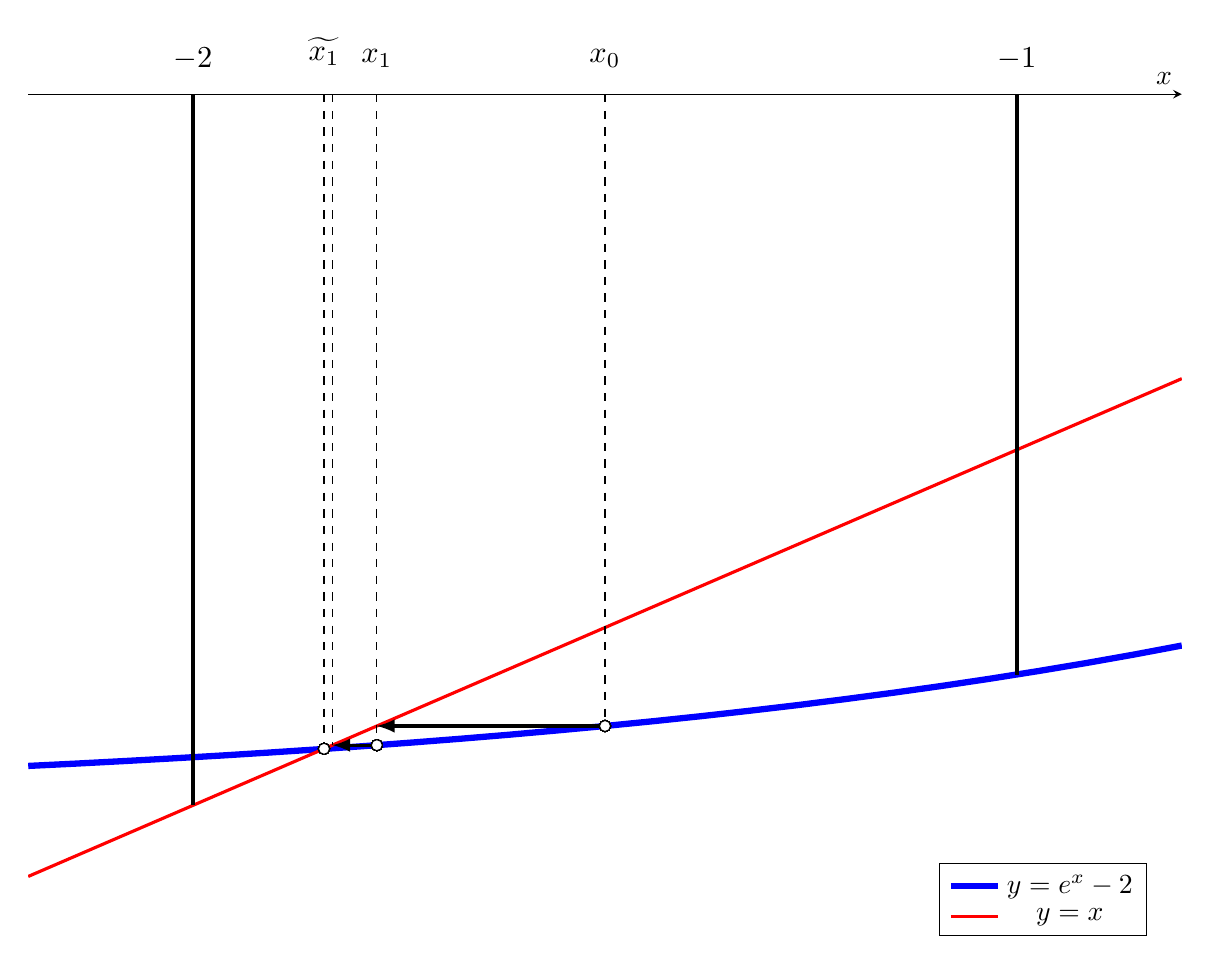
\begin{tikzpicture}
		\begin{axis} [
			height=14cm,
			xlabel = {$x$},
			ylabel = {$y$},
			axis x line = middle,
			hide y axis,
			ymax = 0.3,
			domain = -2.2:-0.8,
			ticks = none,
			legend pos = south east ]

			\coordinate(a) at (-2,0);

			\addplot[color=blue, line width=.08cm]{e^x - 2};
			\addplot[color=red, line width=.04cm]{x};

			\addplot[mark=*,only marks, fill=white] (-1.841,-1.841)
				node[above, pos=1]{};
			\addplot[mark=*,only marks, fill=white] (-1.5,-1.7769)
				node[above, pos=1]{};
			\addplot[mark=*,only marks, fill=white] (-1.7769,-1.8308)
				node[above, pos=1]{};

			\draw[very thick,black] (a) -- (-2,-2);
			\draw[very thick,black] (-1,0) -- (-1,-1.6321);
			\draw[dashed,black] (-1.841,0) -- (-1.841,-1.841);
			\draw[dashed,black] (-1.5,0) -- (-1.5,-1.7769);
			\draw[dashed,black] (-1.7769,0) -- (-1.7769,-1.8308);
			\draw[dashed,black] (-1.8308,0) -- (-1.8308,-1.8308);

			\draw[-latex, black, very thick] (-1.5, -1.7769) -- (-1.7769, -1.7769);
			\draw[-latex, black, very thick] (-1.7769, -1.8308) -- (-1.8308, -1.8308);

			\node[scale=1.1] at (-2,0.1) {$-2$};
			\node[scale=1.1] at (-1,0.1) {$-1$};
			\node[scale=1.1] at (-1.841,0.12) {$\widetilde{x_1}$};
			\node[scale=1.1] at (-1.5,0.1) {$x_0$};
			\node[scale=1.1] at (-1.7769,0.1) {$x_1$};

			\addlegendentry{$y=e^x-2$};
			\addlegendentry{$y=x$};
		\end{axis}
	\end{tikzpicture}

\end{document}
